\begin{figure}[H]
\centering
\resizebox{0.78\linewidth}{!}{%
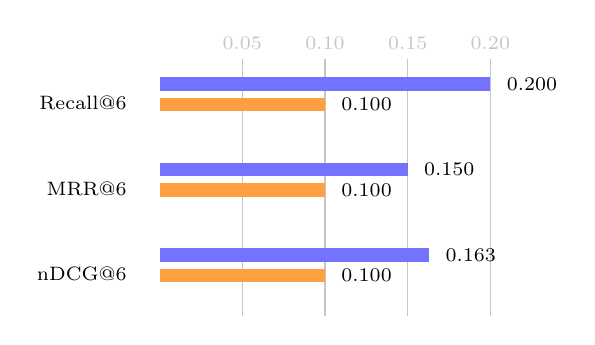
\begin{tikzpicture}[x=21cm,y=0.62cm,font=\scriptsize]
\foreach \x/\lab in {0.05/0.05,0.10/0.10,0.15/0.15,0.20/0.20}
  \draw[gray!45] (\x,0.58) -- (\x,5.85) node[above]{\lab};

\node[anchor=east] at (-0.014,4.95) {Recall@6};
\fill[blue!55] (0,5.20) rectangle (0.20,5.48);
\node[anchor=west] at (0.204,5.34) {0.200};
\fill[orange!75] (0,4.78) rectangle (0.10,5.06);
\node[anchor=west] at (0.104,4.92) {0.100};

\node[anchor=east] at (-0.014,3.20) {MRR@6};
\fill[blue!55] (0,3.45) rectangle (0.15,3.73);
\node[anchor=west] at (0.154,3.59) {0.150};
\fill[orange!75] (0,3.03) rectangle (0.10,3.31);
\node[anchor=west] at (0.104,3.17) {0.100};

\node[anchor=east] at (-0.014,1.45) {nDCG@6};
\fill[blue!55] (0,1.70) rectangle (0.163,1.98);
\node[anchor=west] at (0.167,1.84) {0.163};
\fill[orange!75] (0,1.28) rectangle (0.10,1.56);
\node[anchor=west] at (0.104,1.42) {0.100};
\end{tikzpicture}
}
\caption{Measured pilot retrieval metrics on the first 10 benchmark questions. Blue bars show dense retrieval; orange bars show hybrid rerank. The run used $k=6$ and generated LLM answers.}
\label{fig:retrieval-metrics}
\end{figure}
